%% 
%% Copyright 2019-2020 Elsevier Ltd
%% 
%% This file is part of the 'CAS Bundle'.
%% --------------------------------------
%% 
%% It may be distributed under the conditions of the LaTeX Project Public
%% License, either version 1.2 of this license or (at your option) any
%% later version.  The latest version of this license is in
%%    http://www.latex-project.org/lppl.txt
%% and version 1.2 or later is part of all distributions of LaTeX
%% version 1999/12/01 or later.
%% 
%% The list of all files belonging to the 'CAS Bundle' is
%% given in the file `manifest.txt'.
%% 
%% Template article for cas-dc documentclass for 
%% double column output.

%\documentclass[a4paper,fleqn,longmktitle]{cas-dc}
\documentclass[a4paper,fleqn]{cas-dc}

%\usepackage[numbers]{natbib}
%\usepackage[authoryear]{natbib}
\usepackage[authoryear,longnamesfirst]{natbib}

%%%Author definitions
\def\tsc#1{\csdef{#1}{\textsc{\lowercase{#1}}\xspace}}
\tsc{WGM}
\tsc{QE}
\tsc{EP}
\tsc{PMS}
\tsc{BEC}
\tsc{DE}
%%%

% Uncomment and use as if needed
%\newtheorem{theorem}{Theorem}
%\newtheorem{lemma}[theorem]{Lemma}
%\newdefinition{rmk}{Remark}
%\newproof{pf}{Proof}
%\newproof{pot}{Proof of Theorem \ref{thm}}

\begin{document}
\let\WriteBookmarks\relax
\def\floatpagepagefraction{1}
\def\textpagefraction{.001}

% Short title
\shorttitle{Leveraging social media news}

% Short author
\shortauthors{CV Radhakrishnan et~al.}

% Main title of the paper
\title [mode = title]{This is a specimen $a_b$ title}                      
% Title footnote mark
% eg: \tnotemark[1]
\tnotemark[1,2]

% Title footnote 1.
% eg: \tnotetext[1]{Title footnote text}
% \tnotetext[<tnote number>]{<tnote text>} 
\tnotetext[1]{This document is the results of the research
   project funded by the National Science Foundation.}

\tnotetext[2]{The second title footnote which is a longer text matter
   to fill through the whole text width and overflow into
   another line in the footnotes area of the first page.}


% First author
%
% Options: Use if required
% eg: \author[1,3]{Author Name}[type=editor,
%       style=chinese,
%       auid=000,
%       bioid=1,
%       prefix=Sir,
%       orcid=0000-0000-0000-0000,
%       facebook=<facebook id>,
%       twitter=<twitter id>,
%       linkedin=<linkedin id>,
%       gplus=<gplus id>]
\author[1,3]{CV Radhakrishnan}[type=editor,
                        auid=000,bioid=1,
                        prefix=Sir,
                        role=Researcher,
                        orcid=0000-0001-7511-2910]

% Corresponding author indication
\cormark[1]

% Footnote of the first author
\fnmark[1]

% Email id of the first author
\ead{cvr_1@tug.org.in}

% URL of the first author
\ead[url]{www.cvr.cc, cvr@sayahna.org}

%  Credit authorship
\credit{Conceptualization of this study, Methodology, Software}

% Address/affiliation
\affiliation[1]{organization={Elsevier B.V.},
    addressline={Radarweg 29}, 
    city={Amsterdam},
    % citysep={}, % Uncomment if no comma needed between city and postcode
    postcode={1043 NX}, 
    % state={},
    country={The Netherlands}}

% Second author
\author[2,4]{Han Theh Thanh}[style=chinese]

% Third author
\author[2,3]{CV Rajagopal}[%
   role=Co-ordinator,
   suffix=Jr,
   ]
\fnmark[2]
\ead{cvr3@sayahna.org}
\ead[URL]{www.sayahna.org}

\credit{Data curation, Writing - Original draft preparation}

% Address/affiliation
\affiliation[2]{organization={Sayahna Foundation},
    % addressline={}, 
    city={Jagathy},
    % citysep={}, % Uncomment if no comma needed between city and postcode
    postcode={695014}, 
    state={Trivandrum},
    country={India}}

% Fourth author
\author%
[1,3]
{Rishi T.}
\cormark[2]
\fnmark[1,3]
\ead{rishi@stmdocs.in}
\ead[URL]{www.stmdocs.in}

\affiliation[3]{organization={STM Document Engineering Pvt Ltd.},
    addressline={Mepukada}, 
    city={Malayinkil},
    % citysep={}, % Uncomment if no comma needed between city and postcode
    postcode={695571}, 
    state={Trivandrum},
    country={India}}

% Corresponding author text
\cortext[cor1]{Corresponding author}
\cortext[cor2]{Principal corresponding author}

% Footnote text
\fntext[fn1]{This is the first author footnote. but is common to third
  author as well.}
\fntext[fn2]{Another author footnote, this is a very long footnote and
  it should be a really long footnote. But this footnote is not yet
  sufficiently long enough to make two lines of footnote text.}

% For a title note without a number/mark
\nonumnote{This note has no numbers. In this work we demonstrate $a_b$
  the formation Y\_1 of a new type of polariton on the interface
  between a cuprous oxide slab and a polystyrene micro-sphere placed
  on the slab.
  }

% Here goes the abstract
\begin{abstract}
This template helps you to create a properly formatted \LaTeX\ manuscript.

\noindent\texttt{\textbackslash begin{abstract}} \dots 
\texttt{\textbackslash end{abstract}} and
\verb+\begin{keyword}+ \verb+...+ \verb+\end{keyword}+ 
which
contain the abstract and keywords respectively. 

\noindent Each keyword shall be separated by a \verb+\sep+ command.
\end{abstract}

% Use if graphical abstract is present
% \begin{graphicalabstract}
% 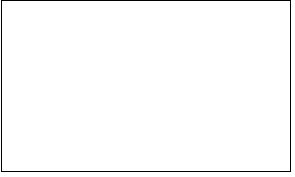
\includegraphics{figs/grabs.pdf}
% \end{graphicalabstract}

% Research highlights
\begin{highlights}
\item Research highlights item 1
\item Research highlights item 2
\item Research highlights item 3
\end{highlights}

% Keywords
% Each keyword is seperated by \sep
\begin{keywords}
quadrupole exciton \sep polariton \sep \WGM \sep \BEC
\end{keywords}


\maketitle

\section{Introduction}

The Elsevier cas-dc class is based on the
standard article class and supports almost all of the functionality of
that class. In addition, it features commands and options to format the
\begin{itemize} \item document style \item baselineskip \item front
matter \item keywords and MSC codes \item theorems, definitions and
proofs \item lables of enumerations \item citation style and labeling.
\end{itemize}

This class depends on the following packages
for its proper functioning:

\begin{enumerate}
\itemsep=0pt
\item {natbib.sty} for citation processing;
\item {geometry.sty} for margin settings;
\item {fleqn.clo} for left aligned equations;
\item {graphicx.sty} for graphics inclusion;
\item {hyperref.sty} optional packages if hyperlinking is
  required in the document;
\end{enumerate}  

All the above packages are part of any
standard \LaTeX{} installation.
Therefore, the users need not be
bothered about downloading any extra packages.

\section{Installation}

The package is available at author resources page at Elsevier
(\url{http://www.elsevier.com/locate/latex}).
The class may be moved or copied to a place, usually,\linebreak
\verb+$TEXMF/tex/latex/elsevier/+, %$%%%%%%%%%%%%%%%%%%%%%%%%%%%%
or a folder which will be read                   
by \LaTeX{} during document compilation.  The \TeX{} file
database needs updation after moving/copying class file.  Usually,
we use commands like \verb+mktexlsr+ or \verb+texhash+ depending
upon the distribution and operating system.

\section{Front matter}

The author names and affiliations could be formatted in two ways:
\begin{enumerate}[(1)]
\item Group the authors per affiliation.
\item Use footnotes to indicate the affiliations.
\end{enumerate}
See the front matter of this document for examples. 
You are recommended to conform your choice to the journal you 
are submitting to.

\section{Bibliography styles}

There are various bibliography styles available. You can select the
style of your choice in the preamble of this document. These styles are
Elsevier styles based on standard styles like Harvard and Vancouver.
Please use Bib\TeX\ to generate your bibliography and include DOIs
whenever available.

Here are two sample references: 
\cite{Fortunato2010}
\cite{Fortunato2010,NewmanGirvan2004}
\cite{Fortunato2010,Vehlowetal2013}

\section{Floats}
{Figures} may be included using the command,\linebreak 
\verb+\includegraphics+ in
combination with or without its several options to further control
graphic. \verb+\includegraphics+ is provided by {graphic[s,x].sty}
which is part of any standard \LaTeX{} distribution.
{graphicx.sty} is loaded by default. \LaTeX{} accepts figures in
the postscript format while pdf\LaTeX{} accepts {*.pdf},
{*.mps} (metapost), {*.jpg} and {*.png} formats. 
pdf\LaTeX{} does not accept graphic files in the postscript format. 

\begin{figure}
	\centering
		
\includegraphics[scale=.75]{figs/Fig1.pdf}
	\caption{The evanescent light - $1S$ quadrupole coupling
	($g_{1,l}$) scaled to the bulk exciton-photon coupling
	($g_{1,2}$). The size parameter $kr_{0}$ is denoted as $x$ and
	the \PMS is placed directly on the cuprous oxide sample ($\delta
	r=0$, See also Table \protect\ref{tbl1}).}
	\label{FIG:1}
\end{figure}


The \verb+table+ environment is handy for marking up tabular
material. If users want to use {multirow.sty},
{array.sty}, etc., to fine control/enhance the tables, they
are welcome to load any package of their choice and
{cas-dc.cls} will work in combination with all loaded
packages.

\begin{table}[width=.9\linewidth,cols=4,pos=h]
\caption{This is a test caption. This is a test caption. This is a test
caption. This is a test caption.}\label{tbl1}
\begin{tabular*}{\tblwidth}{@{} LLLL@{} }
\toprule
Col 1 & Col 2 & Col 3 & Col4\\
\midrule
12345 & 12345 & 123 & 12345 \\
12345 & 12345 & 123 & 12345 \\
12345 & 12345 & 123 & 12345 \\
12345 & 12345 & 123 & 12345 \\
12345 & 12345 & 123 & 12345 \\
\bottomrule
\end{tabular*}
\end{table}

\section[Theorem and ...]{Theorem and theorem like environments}

{cas-dc.cls} provides a few shortcuts to format theorems and
theorem-like environments with ease. In all commands the options that
are used with the \verb+\newtheorem+ command will work exactly in the same
manner. {cas-dc.cls} provides three commands to format theorem or
theorem-like environments: 

\begin{verbatim}
 \newtheorem{theorem}{Theorem}
 \newtheorem{lemma}[theorem]{Lemma}
 \newdefinition{rmk}{Remark}
 \newproof{pf}{Proof}
 \newproof{pot}{Proof of Theorem \ref{thm2}}
\end{verbatim}


The \verb+\newtheorem+ command formats a
theorem in \LaTeX's default style with italicized font, bold font
for theorem heading and theorem number at the right hand side of the
theorem heading.  It also optionally accepts an argument which
will be printed as an extra heading in parentheses. 

\begin{verbatim}
  \begin{theorem} 
   For system (8), consensus can be achieved with 
   $\|T_{\omega z}$ ...
     \begin{eqnarray}\label{10}
     ....
     \end{eqnarray}
  \end{theorem}
\end{verbatim}  


\newtheorem{theorem}{Theorem}

\begin{theorem}
For system (8), consensus can be achieved with 
$\|T_{\omega z}$ ...
\begin{eqnarray}\label{10}
....
\end{eqnarray}
\end{theorem}

The \verb+\newdefinition+ command is the same in
all respects as its \verb+\newtheorem+ counterpart except that
the font shape is roman instead of italic.  Both
\verb+\newdefinition+ and \verb+\newtheorem+ commands
automatically define counters for the environments defined.

The \verb+\newproof+ command defines proof environments with
upright font shape.  No counters are defined. 


\section[Enumerated ...]{Enumerated and Itemized Lists}
{cas-dc.cls} provides an extended list processing macros
which makes the usage a bit more user friendly than the default
\LaTeX{} list macros.   With an optional argument to the
\verb+\begin{enumerate}+ command, you can change the list counter
type and its attributes.

\begin{verbatim}
 \begin{enumerate}[1.]
 \item The enumerate environment starts with an optional
   argument `1.', so that the item counter will be suffixed
   by a period.
 \item You can use `a)' for alphabetical counter and '(i)' 
  for roman counter.
  \begin{enumerate}[a)]
    \item Another level of list with alphabetical counter.
    \item One more item before we start another.
    \item One more item before we start another.
    \item One more item before we start another.
    \item One more item before we start another.
\end{verbatim}

Further, the enhanced list environment allows one to prefix a
string like `step' to all the item numbers.  

\begin{verbatim}
 \begin{enumerate}[Step 1.]
  \item This is the first step of the example list.
  \item Obviously this is the second step.
  \item The final step to wind up this example.
 \end{enumerate}
\end{verbatim}

\section{Cross-references}
In electronic publications, articles may be internally
hyperlinked. Hyperlinks are generated from proper
cross-references in the article.  For example, the words
\textcolor{black!80}{Fig.~1} will never be more than simple text,
whereas the proper cross-reference \verb+\ref{tiger}+ may be
turned into a hyperlink to the figure itself:
\textcolor{blue}{Fig.~1}.  In the same way,
the words \textcolor{blue}{Ref.~[1]} will fail to turn into a
hyperlink; the proper cross-reference is \verb+\cite{Knuth96}+.
Cross-referencing is possible in \LaTeX{} for sections,
subsections, formulae, figures, tables, and literature
references.

\section{Bibliography}

Two bibliographic style files (\verb+*.bst+) are provided ---
{model1-num-names.bst} and {model2-names.bst} --- the first one can be
used for the numbered scheme. This can also be used for the numbered
with new options of {natbib.sty}. The second one is for the author year
scheme. When  you use model2-names.bst, the citation commands will be
like \verb+\citep+,  \verb+\citet+, \verb+\citealt+ etc. However when
you use model1-num-names.bst, you may use only \verb+\cite+ command.

\verb+thebibliography+ environment.  Each reference is a\linebreak
\verb+\bibitem+ and each \verb+\bibitem+ is identified by a label,
by which it can be cited in the text:

\noindent In connection with cross-referencing and
possible future hyperlinking it is not a good idea to collect
more that one literature item in one \verb+\bibitem+.  The
so-called Harvard or author-year style of referencing is enabled
by the \LaTeX{} package {natbib}. With this package the
literature can be cited as follows:

\begin{enumerate}[\textbullet]
\item Parenthetical: \verb+\citep{WB96}+ produces (Wettig \& Brown, 1996).
\item Textual: \verb+\citet{ESG96}+ produces Elson et al. (1996).
\item An affix and part of a reference:\break
\verb+\citep[e.g.][Ch. 2]{Gea97}+ produces (e.g. Governato et
al., 1997, Ch. 2).
\end{enumerate}

In the numbered scheme of citation, \verb+\cite{<label>}+ is used,
since \verb+\citep+ or \verb+\citet+ has no relevance in the numbered
scheme.  {natbib} package is loaded by {cas-dc} with
\verb+numbers+ as default option.  You can change this to author-year
or harvard scheme by adding option \verb+authoryear+ in the class
loading command.  If you want to use more options of the {natbib}
package, you can do so with the \verb+\biboptions+ command.  For
details of various options of the {natbib} package, please take a
look at the {natbib} documentation, which is part of any standard
\LaTeX{} installation.

\appendix
\section{My Appendix}
Appendix sections are coded under \verb+\appendix+.

\verb+\printcredits+ command is used after appendix sections to list 
author credit taxonomy contribution roles tagged using \verb+\credit+ 
in frontmatter.

\printcredits

%% Loading bibliography style file
%\bibliographystyle{model1-num-names}
\bibliographystyle{cas-model2-names}

% Loading bibliography database
\bibliography{cas-refs}


%\vskip3pt

\bio{}
Author biography without author photo.
Author biography. Author biography. Author biography.
Author biography. Author biography. Author biography.
Author biography. Author biography. Author biography.
Author biography. Author biography. Author biography.
Author biography. Author biography. Author biography.
Author biography. Author biography. Author biography.
Author biography. Author biography. Author biography.
Author biography. Author biography. Author biography.
Author biography. Author biography. Author biography.
\endbio

\bio{figs/pic1}
Author biography with author photo.
Author biography. Author biography. Author biography.
Author biography. Author biography. Author biography.
Author biography. Author biography. Author biography.
Author biography. Author biography. Author biography.
Author biography. Author biography. Author biography.
Author biography. Author biography. Author biography.
Author biography. Author biography. Author biography.
Author biography. Author biography. Author biography.
Author biography. Author biography. Author biography.
\endbio

\bio{figs/pic1}
Author biography with author photo.
Author biography. Author biography. Author biography.
Author biography. Author biography. Author biography.
Author biography. Author biography. Author biography.
Author biography. Author biography. Author biography.
\endbio

\end{document}

